\chapter{The binomial distribution}
\label{ch:binomial}

A \textbf{Bernoulli variable} takes on only two values: 0 or 1. For
example:

\begin{enumerate}
\item a coin may land on its head (1) or tail (0);
\item a die may land on $\raisebox{-2pt}{\Cube{6}}$ (1) or not (0);
\item a `wildcat' exploration well may produce petroleum (1) or be dry
  (0).
\end{enumerate}

Consider five gold diggers during the 1849 California gold rush, who
have each purchased a claim in the Sierra Nevada foothills. Geological
evidence suggests that, on average, two thirds of the claims in the
area should contain gold (1), and the remaining third do not (0). The
probability that none of the five prospectors find gold is
\[
P(0\times\mbox{gold}) = P(00000) = (1/3)^5 = 0.0041
\]

The chance that exactly one of the prospectors strikes gold is
\[
P(1\times\mbox{gold}) = P(10000) + P(01000) + P(00100) + P(00010) + P(00001)
\]

\noindent where
\begin{align*}
  P(10000) = & (2/3) (1/3)^4 = 0.0082 \\
  P(01000) = & (1/3) (2/3) (1/3)^3 = 0.0082 \\
  P(00100) = & (1/3)^2 (2/3) (1/3)^2 = 0.0082 \\
  P(00010) = & (1/3)^3 (2/3) (1/3) = 0.0082 \\
  P(00001) = & (1/3)^4 (2/3) = 0.0082
\end{align*}

\noindent so that
\[
P(1\times\mbox{gold}) = \binom{5}{1} (2/3) (1/3)^4 = {5}\times{0.0082} = 0.041
\]

\noindent in which we recognise the binomial coefficient
(Equation~\ref{eq:nchoosek}). Similarly:
\begin{align*}
P(2\times\mbox{gold}) & = \binom{5}{2} (2/3)^2 (1/3)^3 = {10}\times{0.016} = 0.16\\
P(3\times\mbox{gold}) & = \binom{5}{3} (2/3)^3 (1/3)^2 = {10}\times{0.033} = 0.33\\
P(4\times\mbox{gold}) & = \binom{5}{4} (2/3)^4 (1/3) = {5}\times{0.066} = 0.33\\
P(5\times\mbox{gold}) & = \binom{5}{5} (2/3)^5 (1/3)^0 = {1}\times{0.13} = 0.13
\end{align*}

These probabilities form a \textbf{probability mass function} (PMF),
and can be visualised as a bar chart:

\noindent\begin{minipage}[t][][b]{.3\textwidth}
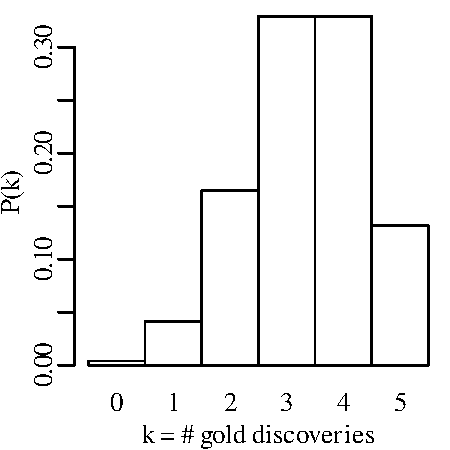
\includegraphics[width=\textwidth]{../figures/goldbarplot.pdf}
\medskip
\end{minipage}
\begin{minipage}[t][][t]{.7\textwidth}
  \captionof{figure}{The probability mass function (PMF) for a
    binomial experiment with a 2/3 chance of success (and a 1/3 chance
    of failure) for five gold prospecting claims. The horizontal axis
    is labelled with the number of claims that produce gold. The
    vertical axis shows the probability of these respective
    outcomes.\medskip}
  \label{fig:goldbar}
\end{minipage}

The generic equation for the PMF of the binomial distribution is
\begin{equation}
  P(k|n,p) = \binom{n}{k} p^k (1-p)^{n-k}
  \label{eq:binom}
\end{equation}

\noindent where $p$ is the probability of success and $k$ is the
number of successes out of $n$ trials. Equivalently, the results can
also be shown as a \textbf{cumulative distribution function} (CDF):
\begin{equation}
  F(x) = P(X \leq x)
  \label{eq:CDF}
\end{equation}

\noindent\begin{minipage}[t][][b]{.3\textwidth}
  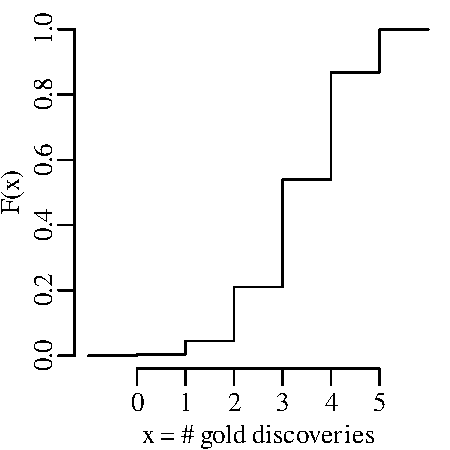
\includegraphics[width=\textwidth]{../figures/goldCDF.pdf}
\end{minipage}
\begin{minipage}[t][][t]{.7\textwidth}
  \captionof{figure}{The cumulative distribution function (CDF) of the
    binomial distribution. This is the running sum of
    Figure~\ref{fig:goldbar}. The horizontal axis is labelled with the
    number of claims that produce gold. The vertical axis shows the
    cumulative probability of these respective outcomes. For example,
    the probability that two or fewer prospectors find gold is 21\%.}
  \label{fig:goldCDF}
\end{minipage}

\section{Parameter estimation}
\label{sec:binompar}

The previous section assumed that the probability of success ($p$ in
Equation~\ref{eq:binom}) is known.  In the real world, this is rarely
the case. In fact, $p$ is usually the parameter whose value we want to
determine based on some data. Consider the general case of $k$
successes among $n$ trials. Then we can estimate $p$ by reformulating
Equation~\ref{eq:binom} in terms of $p$ instead of $k$:
\begin{equation}
  \mathcal{L}(p|n,k) = \binom{n}{k} p^k (1-p)^{n-k}
  \label{eq:Lbinom}
\end{equation}

This is called the \textbf{likelihood function}. The only difference
between the probability mass function (Equation~\ref{eq:binom}) and
the likelihood function (Equation~\ref{eq:Lbinom}) is that former
calculates the probability of an outcome $k$ given the parameters $n$
and $p$, whereas the latter is used to estimate the parameter $p$
given the data $n$ and $k$. The \emph{most likely} value of $p$ given
$n$ and $k$ can be found by maximising $\mathcal{L}(p|n,k)$.  This can
be achieved by taking the derivative of Equation~\ref{eq:Lbinom} with
respect to $p$ and setting it to zero:
\[
\left.\frac{\partial{\mathcal{L}(p|n,k)}}{\partial{p}}\right|_{\hat{p}} = 0
\]

\noindent which gives
\[
\binom{n}{k} k \hat{p}^{k-1} (1-\hat{p})^{n-k} -
\binom{n}{k} \hat{p}^k (n-k) (1-\hat{p})^{n-k-1} = 0
\]

The $\hat{~}$ symbol indicates that $\hat{p}$ is an \emph{estimate}
for the true parameter value $p$, which is unknown. Dividing by
$\binom{n}{k}$ and rearranging:
\[
  k \hat{p}^{k-1} (1-\hat{p})^{n-k} = \hat{p}^k (n-k) (1-\hat{p})^{n-k-1}
\]

Dividing both sides by $\hat{p}^k (1-\hat{p})^{n-k}$:
\[
k (1-\hat{p}) = \hat{p} (n-k)
\]

\noindent which can be solved for $\hat{p}$:
\begin{equation}
  \hat{p} = \frac{k}{n}
  \label{eq:phat}
\end{equation}

Let us apply Equation~\ref{eq:phat} to our gold prospecting example.
Suppose that only two of the five claims produce gold. Then our best
estimate for $p$ given this result is
\[
\hat{p} = \frac{2}{5} = 0.4
\]

So based on this very small dataset, our best estimate for the
abundance of gold in the Sierra Nevada foothills is 40\%. This may be
a trivial result, but it is nevertheless a useful one. The derivation
of Equation~\ref{eq:phat} from Equation~\ref{eq:Lbinom} follows a
recipe that underpins much of mathematical statistics. It is called
the \textbf{method of maximum likelihood}. Of course, the derivation
of parameter estimates is not always as easy as it is for the binomial
case.

\section{Hypothesis tests}
\label{sec:binomH}

Let us continue with our gold prospecting example. Given that only two
of the five prospectors found gold, our best estimate for the
abundance of gold-bearing claims in the prospecting area is $\hat{p} =
2/5$ (40\%). However the introductory paragraph to this chapter
mentioned that geological evidence suggests that 2/3 (67\%) of the
claims should contain gold. Can the discrepancy between the predicted
and the observed number of successes by attributed to bad luck, or
does it mean that the geological estimates were wrong? To answer this
question, we follow a sequence of six steps:

\begin{enumerate}

\item Formulate two hypotheses:\medskip

\noindent\begin{minipage}{.4\textwidth}
  $H_0$ (\textbf{null hypothesis})
  
  \vspace{1em}
  
  $H_{\!A}$ (\textbf{alternative hypothesis}):
\end{minipage}
\begin{minipage}{.2\textwidth}
\end{minipage}
\begin{minipage}{.2\textwidth}
  $p={2/3}$
  
  \vspace{1em}
  
  $p<{2/3}$
\end{minipage}
\begin{minipage}{.2\textwidth}
\end{minipage}\medskip

\item Calculate the \textbf{test statistic} $T$, which in this case is
  the number of successes ($k$).

\item Determine the \textbf{null distribution} of $T$ under
  $H_0$. In our example this is the binomial distribution, as
  shown in Figures~\ref{fig:goldbar} and \ref{fig:goldCDF}. Tabulating
  the PMF and CDF of success:

  \begin{center}
  \begin{tabular}{ccccccc}
    k & 0 & 1 & \textit{2} & 3 & 4 & 5 \\ \hline
    $P(T=k)$ & 0.0041 & 0.0411 & \textit{0.1646} & 0.3292 & 0.3292 & 0.1317 \\
    $P({T}\leq{k})$ & 0.0041 & 0.0453 & \textit{0.2099} & 0.5391 & 0.8683 & 1.0000
  \end{tabular}
  \end{center}

The \textbf{p-value}\footnote{The term `p-value' is not to be confused
  with the value of our unknown binomial parameter $p$. The p-value
  would exist even if we had named the binomial parameter something
  else (e.g., $q$).} is the probability of obtaining test results at
least as extreme as the result actually observed, under the assumption
that the null hypothesis is correct. For our one-sided test, the
p-value is 0.2099, which corresponds with the probability of observing
$k\leq{2}$ successful claims if $p=2/3$.
  
\item Choose a \textbf{significance level $\alpha$}. It is customary
  to choose $\alpha=0.05$.

\item\label{it:rejection} Mark all the outcomes that are incompatible
  with $H_0$.  This \textbf{rejection region} is marked in bold in
  the following table:

  \begin{center}
  \begin{tabular}{ccccccc}
    k & \textbf{0} & \textbf{1} & \textit{2} & 3 & 4 & 5 \\ \hline
    $P(T=k)$ & 0.0041 & 0.0411 & \textit{0.1646} & 0.3292 & 0.3292 & 0.1317 \\
    $P({T}\leq{k})$ & \textbf{0.0041} & \textbf{0.0453} &
    \textit{0.2099} & 0.5391 & 0.8683 & 1.0000
  \end{tabular}
  \end{center}

  $k=0$ and $k=1$ are incompatible with $H_0$ because the
  probability of finding gold in $k\leq{1}$ claims is only 0.0453,
  which is less than $\alpha$. Therefore our rejection region contains
  two values:
  \[
  R = \{0,1\}
  \]

\item\label{it:decision} Reach a \textbf{decision}. Evaluate whether
  the observed outcome for the test statistics falls inside the
  rejection region. If it does, then $H_0$ is rejected in favour
  of $H_{\!A}$. In our example,
  \[
  k=2\notin{R}
  \]

  \noindent which means that we cannot reject $H_0$.
  Alternatively, and equivalently, we can reach the same conclusion by
  observing that the p-value is greater than $\alpha$ (i.e.,
  $0.2099>0.05$). \textit{Note that failure to reject the null
    hypothesis does \underline{not} mean that said hypothesis has been
    \underline{accepted}!}\label{pag:notaccepted}
  
\end{enumerate}

Displaying the rejection region graphically:\medskip

\noindent\begin{minipage}[t][][b]{.6\textwidth}
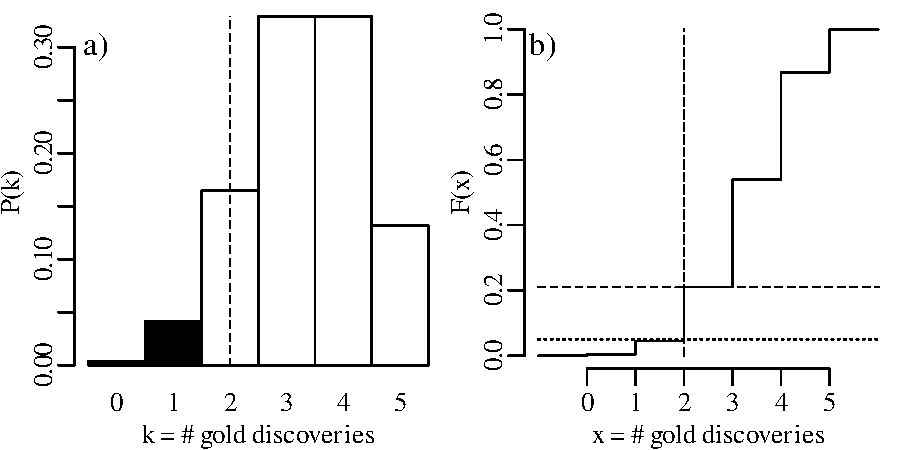
\includegraphics[width=\textwidth]{../figures/1sidedbinomialrejection5.pdf}
\medskip
\end{minipage}
\begin{minipage}[t][][t]{.4\textwidth}
  \captionof{figure}{a) PMF and b) CDF of a binomial null distribution
    with $p=2/3$ and $n=5$. The rejection region is marked in black on
    a).  The horizontal dotted line in b) shows the $\alpha=0.05$
    cutoff mark. The horizontal dashed line in b) marks the p-value
    for $k=2$, which is greater than $\alpha$. Therefore, the null
    hypothesis cannot be rejected.}
  \label{fig:1sidedbinomialrejection5}
\end{minipage}

The above hypothesis test is called a \textbf{one-sided} hypothesis
test, which refers to the fact that $H_{\!A}$ specifies a direction
(`$<$' or `$>$').  Alternatively, we can also formulate a
\textbf{two-sided} hypothesis test:

\begin{enumerate}

\item In this case $H_0$ and $H_{\!A}$ are symmetric:\medskip

\noindent\begin{minipage}{.4\textwidth}
  $H_0$ (null hypothesis)
  
  \vspace{1em}
  
  $H_{\!A}$ (alternative hypothesis):
\end{minipage}
\begin{minipage}{.2\textwidth}
\end{minipage}
\begin{minipage}{.2\textwidth}
  $p=2/3$
  
  \vspace{1em}
  
  ${p}\neq{2/3}$
\end{minipage}
\begin{minipage}{.2\textwidth}
\end{minipage}\medskip

\item The test statistic remains the same as before.

\item We add one line to our table of cumulative outcomes, in order to
  evaluate the high end of the scale as well as its low end:

  \begin{center}
    \begin{tabular}{ccccccc}
      k & 0 & 1 & \textit{2} & 3 & 4 & 5 \\ \hline
      $P(T=k)$ & 0.0041 & 0.0411 & \textit{0.1646} & 0.3292 & 0.3292 & 0.1317 \\
      $P({T}\leq{k})$ & 0.0041 & 0.0453 & \textit{0.2099} &
      0.5391 & 0.8683 & 1.0000 \\
      $P({T}\geq{k})$ & 1.000 & 0.9959 & \textit{0.9547} &
      0.7901 & 0.4609 & 0.1317
    \end{tabular}
  \end{center}
  
\item The significance level is kept the same, but is now evaluated
  twice at $\alpha/2$ to accommodate both tails of the binomial
  distribution.

\item Mark all the outcomes that are incompatible with $H_0$, i.e. all
  the values $k$ with $P(T\leq{k})$ or $P(T\geq{k}) <\alpha/2$.  This
    \textbf{rejection region} is marked in bold in the following
    table:

  \begin{center}
    \begin{tabular}{ccccccc}
      k & \textbf{0} & 1 & \textit{2} & 3 & 4 & 5 \\ \hline
      $P(T=k)$ & 0.0041 & 0.0411 & \textit{0.1646} & 0.3292 & 0.3292 & 0.1317 \\
      $P({T}\leq{k})$ & \textbf{0.0041} & 0.0453 &
      \textit{0.2099} & 0.5391 & 0.8683 & 1.0000 \\
      $P({T}\geq{k})$ & 1.000 & 0.9959 & \textit{0.9547} & 0.7901 & 0.4609 & 0.1317
    \end{tabular}
  \end{center}

  \noindent which yields a smaller rejection region than before,
  because $P(T\leq{1})=0.0453$, which is greater than
  $\alpha/2=0.025$.  The same is true for $P(T\geq{k})$ for any
  $k$. Therefore:
  \[
  R = \{0\}
  \]

\item Again, we fail to reject $H_0$, which means that the
  observed $k/n=2/5$ success rate does not rule out the possibility
  that the true value of $p=2/3$, and that the geologists were
  therefore correct.
  
\end{enumerate}

Displaying the two-sided hypothesis test graphically:\medskip

\noindent\begin{minipage}[t][][b]{.6\textwidth}
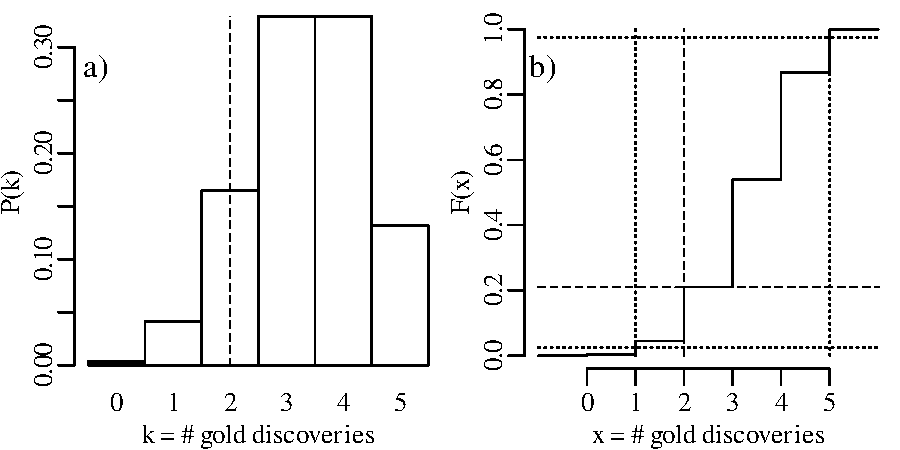
\includegraphics[width=\textwidth]{../figures/2sidedbinomialrejection5.pdf}
\medskip
\end{minipage}
\begin{minipage}[t][][t]{.4\textwidth}
  \captionof{figure}{a) the same PMF and b) CDF as
    Figure~\ref{fig:1sidedbinomialrejection5}. Horizontal dotted lines
    mark $\alpha/2=0.025$ and $(1-\alpha/2)=0.975$. Their
    intersections with the CDF are shown as vertical dotted lines and
    mark the outer edges of the rejection region.  The dashed lines
    mark the observed value and probability, which fall outside the
    rejection region.}
  \label{fig:2sidedbinomialrejection5}
\end{minipage}

Again, $H_0$ cannot be rejected at an $\alpha=0.05$ significance
level.  So in this case the one-sided and two-sided hypothesis tests
produce exactly the same result, as the observed value $k=2$ is not in
the rejection region for either test. However this is not always the
case, as will be shown next.

\section{Statistical power}
\label{sec:power}

Suppose that not five but fifteen gold prospectors had purchased a
claim in the same area as before. And suppose that six of these
prospectors had struck gold. Then the maximum likelihood estimate for
$p$ is:
\[
\hat{p} = \frac{6}{15} = 0.4
\]

\noindent which is the same as before. The one-sided hypothesis test
($H_0: p={2/3}$ vs. $H_{\!A}: p<2/3$) proceeds as before, but leads to
a different table of probabilities:

\begin{center}
  \begin{tabular}{c@{\gap}c@{\gap}c@{\gap}c@{\gap}c@{\gap}c@{\gap}c@{\gap}c@{\gap}c}
    k & \textbf{0} & \textbf{1} & \textbf{2} & \textbf{3} & \textbf{4}
    & \textbf{5} & \textbf{\textit{6}} & 7 \\ \hline $P(T=k)$ &
    7.0$\times{10}^{-8}$ & 2.1$\times{10}^{-6}$ & 2.9$\times{10}^{-5}$
    & 2.5$\times{10}^{-4}$ & 0.0015 & 0.0067 & \textit{0.0223} & 0.0574 \\
    $P({T}\leq{k})$ & \textbf{7.0}$\mathbf{\times{10}^{-8}}$
    & \textbf{2.2}$\mathbf{\times{10}^{-6}}$ &
    \textbf{3.1}$\mathbf{\times{10}^{-5}}$ &
    \textbf{2.8}$\mathbf{\times{10}^{-4}}$ & \textbf{0.0018} &
    \textbf{0.0085} & \textbf{\textit{0.0308}} & 0.0882 \\
    k & 8 & 9 & 10 & 11 & 12 & 13 & 14 & 15 \\
    \hline $P(T=k)$ & 0.1148 & 0.1786 & 0.2143
    & 0.1948 & 0.1299 & 0.0599 & 0.0171 & 0.0023 \\
    $P({T}\leq{k})$ & 0.2030 & 0.3816 & 0.5959 & 0.7908 &
    0.9206 & 0.9806 & 0.9977 & 1.0000
  \end{tabular}
\end{center}

The rejection region (bold) consists of
\begin{equation}
  R=\{0,1,2,3,4,5,6\}
  \label{eq:1sidedbinomtest15}
\end{equation}

\noindent which includes $k=6$. Therefore $H_0$ is rejected.

\noindent\begin{minipage}[t][][b]{.6\textwidth}
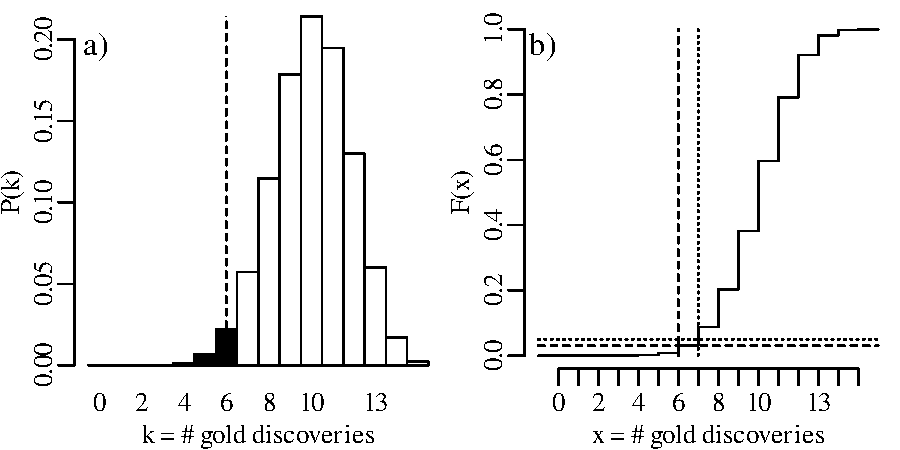
\includegraphics[width=\textwidth]{../figures/1sidedbinomialrejection15.pdf}
\medskip
\end{minipage}
\begin{minipage}[t][][t]{.4\textwidth}
  \captionof{figure}{a) PMF and b) CDF of a binomial distribution with
    $p={2/3}$ and $n=15$. The vertical dashed lines mark the
    observation ($k=6$). They fall in the black area of the bar chart,
    and to the left of the dotted line in the CDF, which marks the
    edge of the rejection region. Therefore, $H_0$ fails the one-sided
    test.}
  \label{fig:1sidedbinomialrejection15}
\end{minipage}

For the two-sided hypothesis test ($H_0: p={2/3}$ vs. $H_{\!A}:
p\neq{2/3}$):

\begin{center}
\begin{tabular}{c@{\gap}c@{\gap}c@{\gap}c@{\gap}c@{\gap}c@{\gap}c@{\gap}c@{\gap}c}
    k & \textbf{0} & \textbf{1} & \textbf{2} & \textbf{3} & \textbf{4}
    & \textbf{5} & \textit{6} & 7 \\ \hline $P(T=k)$ &
    7.0$\times{10}^{-8}$ & 2.1$\times{10}^{-6}$ & 2.9$\times{10}^{-5}$
    & 2.5$\times{10}^{-4}$ & 0.0015 & 0.0067 & \textit{0.0223} & 0.0574 \\
    $P({T}\leq{k})$ & \textbf{7.0}$\mathbf{\times{10}^{-8}}$ &
    \textbf{2.2}$\mathbf{\times{10}^{-6}}$ &
    \textbf{3.1}$\mathbf{\times{10}^{-5}}$ &
    \textbf{2.8}$\mathbf{\times{10}^{-4}}$ & \textbf{0.0018} &
    \textbf{0.0085} & \textit{0.0308} & 0.0882 \\
    $P({T}\geq{k})$ & 1.0000 &
    1-7.0$\times{10}^{-8}$ & 1-2.2$\times{10}^{-6}$ &
    1-3.1$\times{10}^{-5}$ & 1-2.8$\times{10}^{-4}$ & 0.9982 & \textit{0.9915}
    & 0.9692 \\ k & 8 & 9 & 10 & 11 & 12 & 13 & \textbf{14} & \textbf{15} \\ \hline
    $P(T=k)$ & 0.1148 & 0.1786 & 0.2143 & 0.1948
    & 0.1299 & 0.0599 & 0.0171 & 0.0023 \\
    $P({T}\leq{k})$ & 0.2030 &
    0.3816 & 0.5959 & 0.7908 & 0.9206 & 0.9806 & 0.9977 & 1.0000 \\
    $P({T}\geq{k})$ & 0.9118 & 0.7970 & 0.6184 & 0.4041 & 0.2092 &
    0.0794 & \textbf{0.0194} & \textbf{0.0023}
\end{tabular}
\end{center}

The rejection region (which includes both tails of the distribution)
is:
\begin{equation}
  R=\{0,1,2,3,4,5,14,15\}
  \label{eq:2sidedbinomtest15}
\end{equation}

This region does \emph{not} include $k=6$. Therefore we \emph{cannot}
reject the two-sided null hypothesis that $p=2/3$ at
$\alpha=0.05$.\medskip

\noindent\begin{minipage}[t][][b]{.6\textwidth}
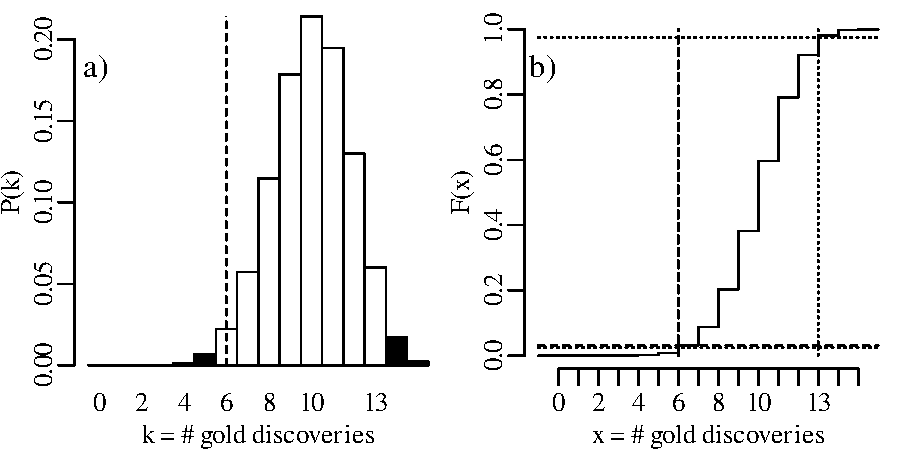
\includegraphics[width=\textwidth]{../figures/2sidedbinomialrejection15.pdf}
\medskip
\end{minipage}
\begin{minipage}[t][][t]{.4\textwidth}
  \captionof{figure}{a) PMF and b) CDF of the binomial distribution
    with $p=2/3$ and $n=15$.  The dotted lines mark the
    $\alpha/2=0.025$ and $(1-\alpha/2)=0.975$ levels and
    quantiles. The dashed lines mark the observed value ($k=6$), which
    falls outside the rejection region.  Therefore $H_0$ does not fail
    the two-sided test.}
  \label{fig:2sidedbinomialrejection15}
\end{minipage}

Let us increase our `sample size' (number of prospectors) even more,
from 15 to 30, and suppose once again that only 40\% of these found
gold even though the geological evidence suggested that this should be
67\%. The lookup table of probabilities would be quite large, so we
will just show the distributions graphically:\medskip

\noindent\begin{minipage}[t][][b]{.65\textwidth}
  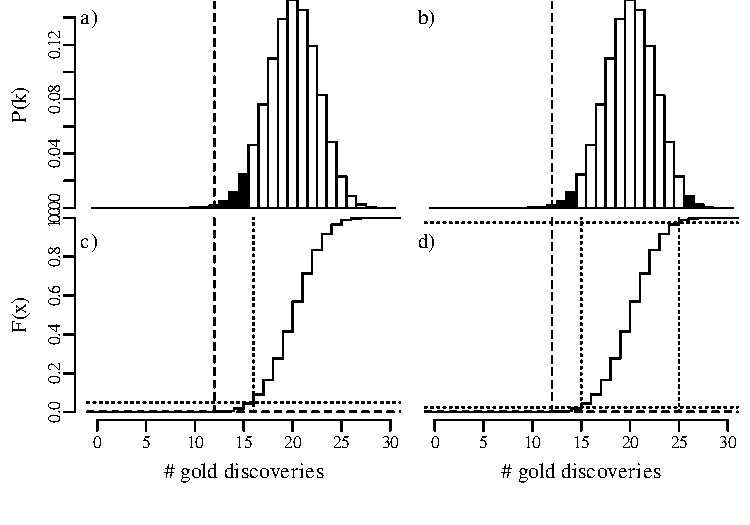
\includegraphics[width=\textwidth]{../figures/binomialrejection30.pdf}
\end{minipage}
\begin{minipage}[t][][t]{.35\textwidth}
  \captionof{figure}{The PMF (a \& b) and CDF (c \& d) for a binomial
    distribution with $p=2/3$ and $n=30$, illustrating a one-sided (a
    \& c) and two-sided (b \& d) test. The vertical dashed lines mark
    the observation $k=12$, which falls inside the rejection regions
    marked in black (a \& b), and outside the cutoff limits defined by
    the vertical dotted lines (c \& d).}
  \label{fig:binomialrejection30}
\end{minipage}

In summary, we have compared the same outcome of 40\% successes with
the null hypothesis $p=2/3$, using three different sample sizes ($n$):

\begin{enumerate}
  \item Both the one-sided and the two-sided hypothesis tests failed
    to reject the null hypothesis for $n=5$ prospectors.
  \item Increasing the number of prospectors to $n=15$ leads to a
    rejection of $H_0$ using the one-sided test but failure to reject
    $H_0$ using the two-sided test.
  \item Further increasing our sample size to $n=30$ whilst still
    keeping the percentage of success the same leads to a firm
    rejection of $H_0$ using both the one-sided and the two-sided
    test.
\end{enumerate}

In statistical terms, the increase in sample size has increased the
`power' of the test to reject the hypothesis test. A formal
mathemathical definition of this concept will be given in
Section~\ref{sec:typeI&II}.

\section{Type-I and type-II errors}
\label{sec:typeI&II}

There are four possible outcomes for a hypothesis test, which can be
organised in a ${2}\times{2}$ table:

\begin{center}
\begin{tabular}{c|cc}
  $H_0$ is ... & false & true \\ \hline
  rejected & correct decision & Type-I error \\
  not rejected & Type-II error & correct decision
\end{tabular}
\end{center}

To appreciate the difference between the two types of errors in this
table, it may be useful to compare statistical hypothesis testing with
a legal analogue. The jury in a court of justice faces a situation
that is similar to that of a statistical hypothesis test. They are
faced with a suspect who has either committed a crime or not, and they
must decide whether to sentence this person or acquit them.  In this
case our `null hypothesis' is that the accused is innocent.  The jury
then needs decide whether there is enough evidence to reject this
hypothesis in favour of the alternative hypothesis, which is that the
accused is guilty. Casting this process in a second ${2}\times{2}$
table:

\begin{center}
\begin{tabular}{c|cc}
  the accused is ... & guilty & innocent \\ \hline
  convicted & correct decision & Type-I error \\
  acquitted & Type-II error & correct decision
\end{tabular}
\end{center}

A \textbf{type-I error} is committed when a true null hypothesis test
is erroneously rejected. This is akin to putting an innocent person in
prison. For our gold prospecting example, this means that we reject
the expert opinion of the geologist (whose assessment indicated a 2/3
chance of finding gold) when this geologist is in fact
correct.\medskip

A \textbf{type-II error} is committed when we fail to reject a false
null hypothesis.  This is akin to letting a guilty person get away
with a crime for lack of evidence. In the geological example, this
means that we conclude that the geological assessment is right despite
it being wrong.\medskip

The probability of committing a type-I error is controlled by one
parameter:

\begin{enumerate}
\item {\bf The confidence level $\alpha$}
  
  Using the customary value of $\alpha=0.05$, there is a 5\% chance of
  committing a type-I error. So even if the null hypothesis is
  correct, then we would still expect to reject it once every 20
  times. This may be acceptable in geological studies, but probably
  not in the legal system! The principle that guilt must be proven
  ``beyond any reasonable doubt'' is akin to choosing a very small
  significance level ($\alpha\ll{0.05}$). However it is never possible
  to enforce $\alpha=0$ unless all suspects are aquitted, so it is
  inevitable that some innocent people are convicted.
\end{enumerate}

The probability of committing a type-II error ($\beta$) depends on two
things:

\begin{enumerate}
\item{\bf The degree to which $H_0$ is false}
  
  In our geological example, 40\% of the prospectors found gold in
  their claim, so there clearly was some gold present in the
  area. Suppose that the actual abundance of gold in the prospecting
  area was indeed 40\% ($p=2/5$) instead of $p=2/3$.  Then the
  expected distribution of outcomes would follow a binomial
  distribution with $p=2/5$. As shown in Section~\ref{sec:binomH}, the
  rejection region for the one-sided hypothesis test of $H_0: p=2/3$
  vs. $H_{\!A}: p<2/3$ is $R=\{0,1\}$ for $n=5$. If the actual value
  for $p$ is 2/5, then the probability of observing a value for $k$
  that falls in this rejection region is $P(k<2|n=5,p=2/5)=0.34$. This
  is known as the \textbf{power} of the statistical test. The
  probability of committing a type-II error is given by:
  
  \begin{equation}
    \beta = 1 - \mbox{power} = 0.66
  \end{equation}

  Next, suppose that the true probability of finding gold is even
  lower, at $p=1/5$. Under this alternative distribution, the
  probability of finding gold in ${k}\leq{1}$ out of $n=5$ claims
  (i.e., the power) increases to 74\%. Therefore, the probability of
  committing a type-II error has dropped to only 26\%.

  Finally, consider an end member situation in which the prospecting
  area does not contain any gold at all ($p=0$). Then the probability
  of finding gold is obviously zero, because $F(x=2)=0$. Under this
  trivial scenario, the power of the test is 100\%, and the
  probability of committing a type-II error is zero.

  Plotting these results graphically:

  \noindent\begin{minipage}[t][][b]{\linewidth}
    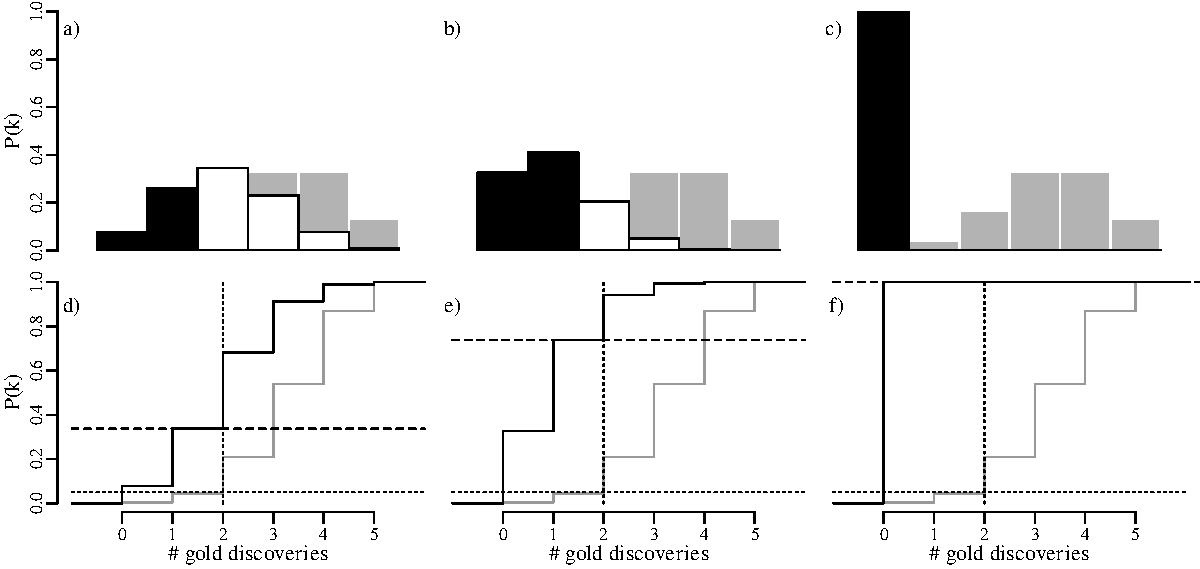
\includegraphics[width=\textwidth]{../figures/binompower1.pdf}
  \end{minipage}
  \begin{minipage}[t][][t]{\linewidth}
  \captionof{figure}{a) -- c) PMFs of the binomial null distribution
    with $p=2/3$ ($H_0$, grey, background) and alternative
    distributions ($H_{\!A}$, black and white, foreground) with a)
    $p=2/5$, b) $p=1/5$ and c) $p=0$. Sample size is $n=5$ for all
    cases.  d) -- f) CDFs for the null distribution (grey) and the
    alternative distribution (black). The horizontal dotted lines mark
    $\alpha=0.05$.  Their intersections with the CDF of the null
    distribution are marked by vertical dotted lines. The areas to the
    left of these lines define the rejection region under a one-sided
    test and are marked in black in the PMFs of the alternative
    distributions (a -- c). The dashed horizontal lines mark the
    intersection of the rejection boundary with the CDF of the
    alternative distribution. They mark the power of the statistical
    test ($1-\beta$).  Power clearly increases as the alternative
    distribution drifts away from the null distribution.}
  \label{fig:binompower1}
  \end{minipage}

\item{\bf Sample size}

  The effect of sample size was already discussed in
  Section~\ref{sec:power}. Comparing the predicted outcomes for the
  null hypothesis $H_0: p=2/3$ to those of the alternative hypothesis
  $H_{\!A}: p=2/5$ for sample sizes of $n=5$, 15 and 30:

  \begin{minipage}[t][][b]{\linewidth}
    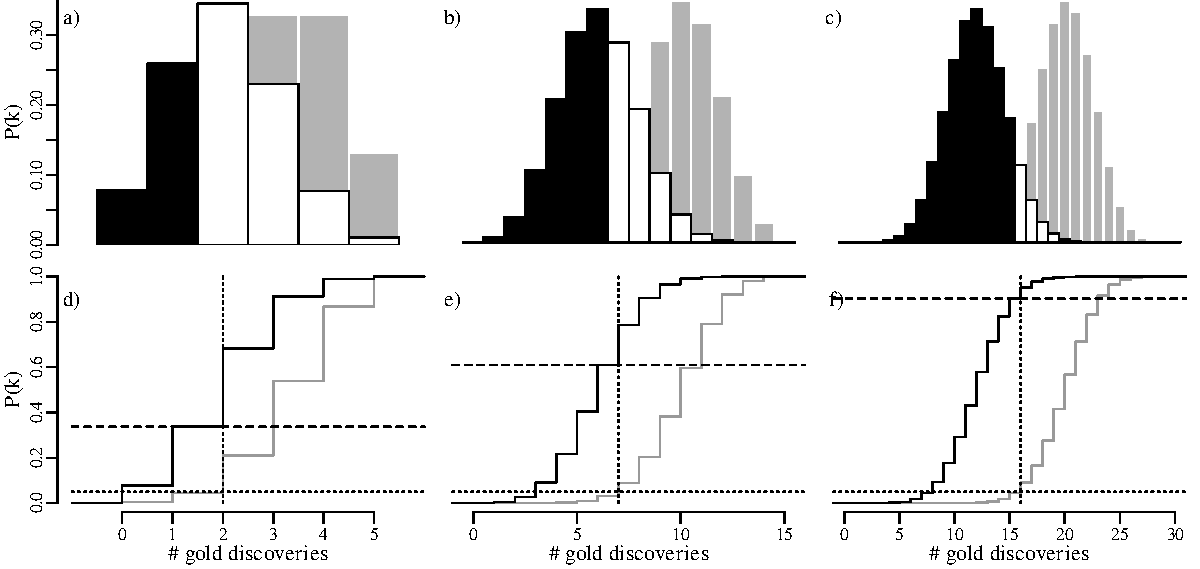
\includegraphics[width=\textwidth]{../figures/binompower2.pdf}
  \end{minipage}
  \begin{minipage}[t][][t]{\linewidth}
    \captionof{figure}{a) -- c) PMFs of binomial distributions with
      $p=2/3$ ($H_0$, grey, background) and $p=2/5$ ($H_{\!A}$, black
      and white, foreground), for sample sizes of a) $n=5$, b) $n=15$
      and c) $n=30$.  d) -- f) CDFs for the null distribution (grey)
      and the alternative distribution (black). The horizontal dotted
      lines mark $\alpha=0.05$, corresponding to a one-sided test.
      Their intersections with the CDF of the null distribution are
      marked by vertical dotted lines. The area to the left of these
      lines define the rejection region and are marked in black in the
      bar chart. The larger the sample size, the easier it is to
      reject $H_0$. The dashed horizontal lines mark the intersection
      of the rejection region with the CDF of the alternative
      distribution. These mark the power of the statistical test
      ($1-\beta$).  Power clearly increases with sample size.}
    \label{fig:binompower2}
  \end{minipage}

\end{enumerate}

\section{Pitfalls of statistical hypothesis testing}
\label{sec:pitfalls}

\hspace{\parindent}\textit{All hypotheses are wrong ... in some decimal place}
\hfill-- John Tukey (paraphrased)\medskip

\textit{All models are wrong, but some are useful}
\hfill-- George Box\medskip

Statistical tests provide a rigorous mathematical framework to assess
the validity of a hypothesis. It is not difficult to see the appeal of
this approach to scientists, including geologists. The scientific
method is based on three simple steps:

\begin{enumerate}
\item Formulate a hypothesis.
\item Design an experiment to test said hypothesis.
\item Carry out the experiment and check to see if it matches the prediction.
\end{enumerate}

It is rarely possible to prove scientific hypotheses. We can only
\emph{disprove} them. New knowledge is gained when the results of an
experiment do not match the expectations. For example:

\begin{enumerate}
\item Hypothesis: Earth's lower mantle is made of olivine.
\item Test: Study the stability of olivine at lower mantle pressures
  (24-136~GPa).
\item Result: Olivine is not stable at lower mantle pressures.
\end{enumerate}

From this experiment we still don't know what the lower mantle is made
of.  But at least we know that it is \emph{not} olivine. Let us
contrast this outcome with a second type of hypothesis:

\begin{enumerate}
\item Hypothesis: Earth's lower mantle is made of perovskite.
\item Test: Study the stability of perovskite at lower mantle
  pressures.
\item Result: Perovskite is stable at lower mantle pressures.
\end{enumerate}

What have we learned from this experiment? Not much. We certainly did
not prove that Earth's lower mantle consists of perovskite. There are
lots of other minerals that are stable at lower mantle pressures. The
only thing that we can say is that the null hypothesis has survived to
live another day. The scientific method is strikingly similar to the
way in which a statistical hypothesis test is carried out. A null
hypothesis, like a scientific hypothesis, cannot be proven. It can
only be disproved. Rejection of a null hypothesis is the best outcome,
because it is the only outcome that teaches us something new. Our
understanding of the natural world continues to improve by falsifying
current hypotheses using scientific experiments, which leads to
revised hypotheses that are closer to the truth.
\medskip

It may seem natural to use the statistical approach to test scientific
hypotheses. However doing so is not without dangers. To explain these
dangers, let us go back to the power analysis of
Section~\ref{sec:power}. The power of our hypothesis test to reject
$H_0: p=2/3$ increases with sample size. A small sample may be
sufficient to detect large deviations from the null
hypothesis. Smaller deviations require larger sample sizes. But no
matter how small the violation of the null hypothesis is, there always
exists a sample size that is large enough to detect it.\medskip

Statistical tests are an effective way to evaluate mathematical
hypotheses. They are less useful for scientific hypotheses.  There is
a profound difference between mathematical and scientific
hypotheses. Whereas a mathematical hypothesis is either `right' or
`wrong', scientific hypotheses are always `somewhat wrong'.
Considering our gold prospecting example, it would be unreasonable to
expect that $p$ is exactly equal to 2/3, down to the
100\textsuperscript{th} significant digit.  Estimating the proportion
of gold in the area to be within 10\% of the truth would already be a
remarkable achievement. Yet given enough data, there will always come
a point where the geological prediction is disproved. Given a large
enough dataset, even a 1\% deviation from the predicted value would
yield an unacceptably small p-value:

\noindent\begin{minipage}[t][][b]{.45\textwidth}
  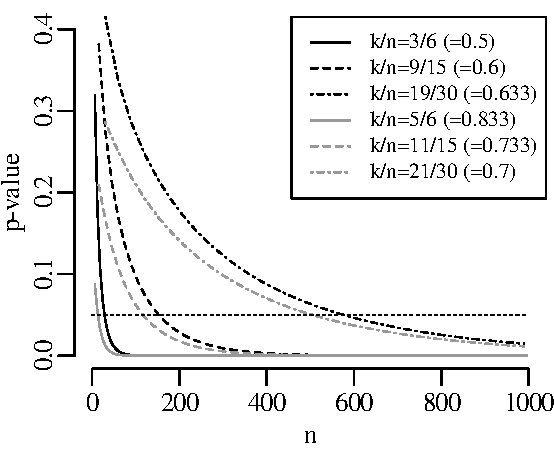
\includegraphics[width=\textwidth]{../figures/binompvsn.pdf}
\end{minipage}
\begin{minipage}[t][][t]{.55\textwidth}
  \captionof{figure}{The p-values of a binomial test comparing the
    null hypothesis $H_0: p=2/3$ with the alternative hypothesis $H_a:
    p<2/3$, for four parameter estimates $\hat{p}$, over a range of
    sample sizes. For each $\hat{p}$, let the outcome $k$ be the
    closest integer to $n\hat{p}$, so that $k/n\approx\hat{p}$. The
    horizontal dotted line marks the 5\% significance level. No matter
    how little the observed $k/n$-ratio differs from 2/3
    $(\approx{0.67})$, this difference always becomes `significant'
    given a large enough sample.}
  \label{fig:binomnvsp}
\end{minipage}

As another example, suppose that we have analysed the mineralogical
composition of two samples of sand that were collected 10~cm apart on
the same beach. Our null hypothesis is that the composition of the two
samples is the same. Plausible though this hypothesis may seem, it
will always be possible to reject it, provided that enough grains are
analysed. We may need to classify a hundred, a thousand or even a
million grains from each sample, but at some point a `statistically
significant' difference will be found. Given a large enough sample,
even the tiniest hydraulic sorting effect becomes detectable.\medskip

In conclusion, formalised hypothesis tests are of limited use in
science.  There are just two exceptions in which they do serve a
useful purpose:

\begin{enumerate}
\item If a statistical test fails to reject the null hypothesis, then
  this indicates that the sample size is too small to find a
  meaningful effect. In this context the statistical test protects us
  against over-interpreting our data.
\item We can calculate the sample size that would be required to
  detect a pre-specified deviation from the null hypothesis, for the
  given type-1 and type-2 thresholds (i.e., $\alpha$ and $\beta$).
  This approach is used in the pharmaceutical industry to test the
  efficacy of drugs. However it is seldom or never available to
  geologists.
\end{enumerate}

\section{Confidence intervals}
\label{sec:binomCI}

The previous section showed that simple binary hypothesis tests are of
limited use in geology. The question that is relevant to scientists is
not so much whether a hypothesis is wrong, but rather \emph{how wrong}
it is. In the context of our gold prospecting example, there is little
use in testing whether $p$ is exactly equal to $2/3$. In reality, $p$
is \emph{unknown}. It is far more useful to actually estimate $p$ and
to quantify the statistical uncertainty associated with it.\medskip

Equation~\ref{eq:phat} showed that, given $k$ successful claims among
$n$ total claims, the \emph{most likely} estimate for $p$ is $k/n$.
For example, if we observe $k=2$ successful claims among $n=5$ trials,
then our best estimate for the abundance of gold is $\hat{p}=2/5$.
However this does not rule out other values. Let us now explore all
possible values for $p$ that are compatible with the observed $k=2$
successful claims:

\begin{enumerate}
\item{\bf p=0?} If $p=0$, then the outcome that $k=2$ would be
  impossible.  So $p=0$ can be ruled out.
\item{\bf p=0.1?} The probability of observing ${k}\geq{2}$ successful
  claims if $p=0.1$ is given by:
  \[
  P({k}\geq{2}|p=0.1,n=5) =
  \sum\limits_{i=2}^{5}\binom{5}{i}(0.1)^i(0.9)^{n-i} = 0.081
  \]
  
  which is greater than $\alpha/2$. Consequently, the observation
  $k=2$ falls outside the rejection region of the two-sided hypothesis
  test, and the proposed parameter value $p=0.1$ is deemed compatible
  with the observation.
\item{\bf p=2/5?} This is our maximum likelihood estimate for $p$.  It
  is definitely possible that this is the true value.
\item{\bf p=2/3?} Figures~\ref{fig:binompower1}.a) and d) show that
  there is a greater than 2.5\% chance of observing 2 or fewer
  successful claims if the true value of $p$ is $2/3$. So $p=2/3$
  remains possible.
\item{\bf p=0.9?} The probability of observing ${k}\leq{2}$ successful
  claims if $p=0.9$ is given by:
  \[
  P({k}\leq{2}|p=0.9,n=5) =
  \sum\limits_{i=0}^{2}\binom{5}{i}(0.9)^i(0.1)^{n-i} = 0.0086
  \]
  which is less than the $\alpha/2$ cutoff, and so $p=0.9$ is
  \emph{not} compatible with the observation.
\item{\bf p=1?} If $p=1$, then 100\% of the claims should contain
  gold. This is incompatible with the observation that $k=2$.
  Therefore $p=1$ can be ruled out.
\end{enumerate}

The set of all values of $p$ that are compatible with the observed
outcome $k=2$ forms a \textbf{confidence interval}. Using an iterative
process, it can be shown that the lower and upper limits of this
interval are given by:
\[
\mbox{C.I.}(p|k=2,n=5) = [0.053, 0.85]
\]

\noindent\begin{minipage}[t][][b]{.65\textwidth}
  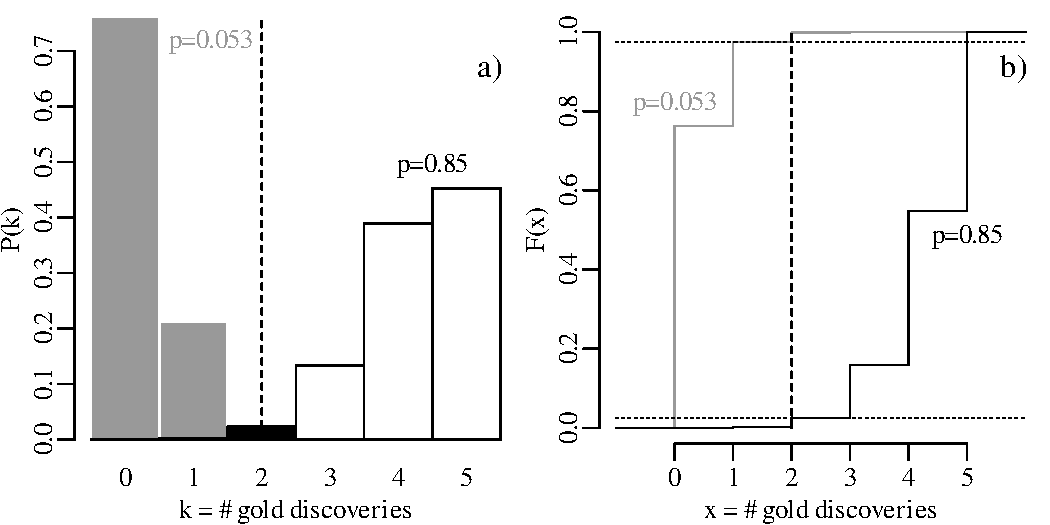
\includegraphics[width=\textwidth]{../figures/binomcik2n5.pdf}\medskip
\end{minipage}
\begin{minipage}[t][][t]{.35\textwidth}
  \captionof{figure}{a) the PMFs and b) CDFs of the binomial parameter
    $p$ given $k=2$ successful claims (dashed lines) out of $n=5$
    (i.e., $\hat{p}=0.4$), for the lower ($p=0.053$, grey) and upper
    ($p=0.85$) limits of a 95\% confidence interval. Dotted horizontal
    lines mark the 0.025 and 0.975 confidence levels.\medskip}
  \label{fig:binomcik2n5}
\end{minipage}

Repeating this procedure for a different result, for example $k=4$,
yields a different confidence interval, namely:
\[
\mbox{C.I.}(p|k=4,n=5) = [0.284, 0.995]
\]

\noindent\begin{minipage}[t][][b]{.65\textwidth}
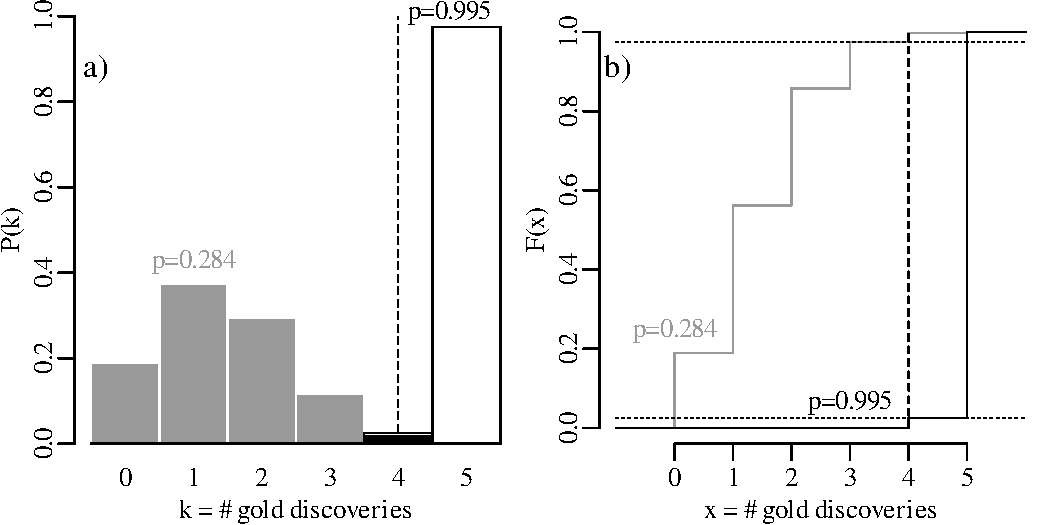
\includegraphics[width=\textwidth]{../figures/binomcik4n5.pdf}
\medskip
\end{minipage}
\begin{minipage}[t][][t]{.35\textwidth}
  \captionof{figure}{The same as Figure~\ref{fig:binomcik2n5}, but for
    $k=4$ successful claims (dashed lines) out of $n=5$ trials (i.e.,
    $\hat{p}=0.8$).\medskip}
  \label{fig:binomcik4n5}
\end{minipage}

What happens if we increase the sample size from $n=5$ to $n=30$, and
the number of successful claims from $k=2$ to $k=12$?  Then the
maximum likelihood estimate remains $\hat{p}=2/5$ as in our first
example, but the 95\% confidence interval narrows down to
\[
\mbox{C.I.}(p|k=12,n=30) = [0.23, 0.59]
\]

\noindent\begin{minipage}[t][][b]{.65\textwidth}
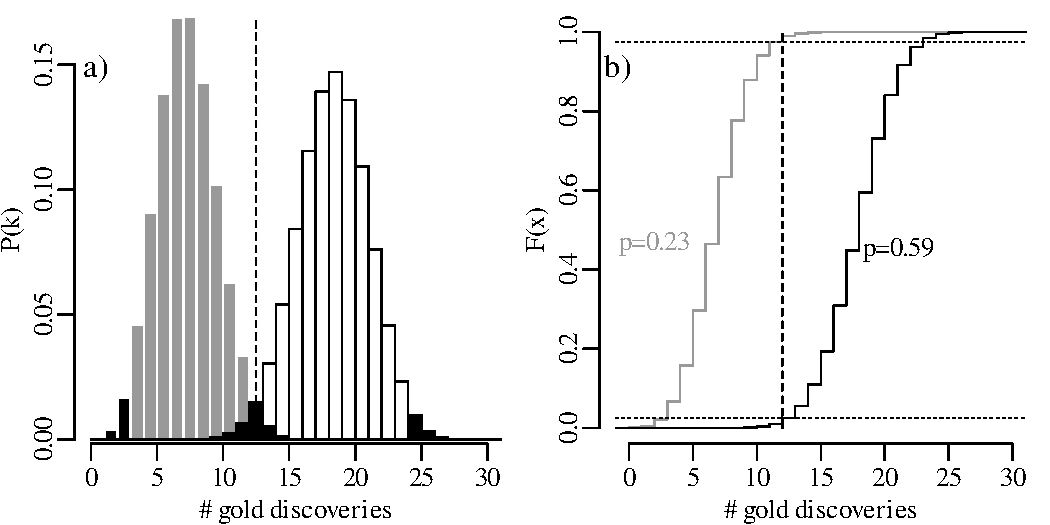
\includegraphics[width=\textwidth]{../figures/binomcik12n30.pdf}
\medskip
\end{minipage}
\begin{minipage}[t][][t]{.35\textwidth}
  \captionof{figure}{The same as Figure~\ref{fig:binomcik2n5}, but for
    $k=12$ successful claims (dashed lines) out of $n=30$ trials
    (i.e., $\hat{p}=0.4$).\medskip}
  \label{fig:binomcik12n30}
\end{minipage}

To further explore the trend of decreasing confidence interval width
with increasing sample size, let us evaluate the 95\% confidence
intervals for $\hat{p}=k/n$ estimates of 2/3 and 1/5, respectively,
over a range of sample sizes between $n=3$ and $n=300$:\medskip

\noindent\begin{minipage}[t][][b]{.65\textwidth}
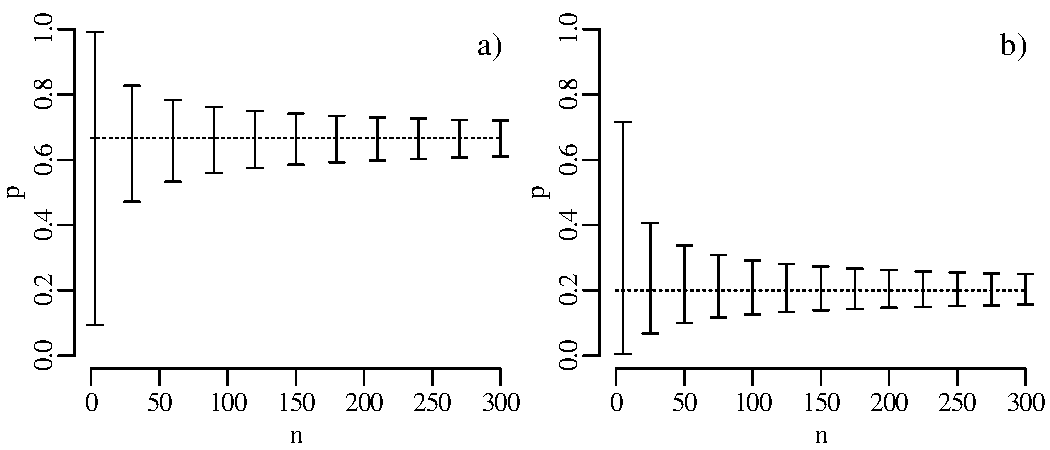
\includegraphics[width=\textwidth]{../figures/binomcivsn.pdf}
\medskip
\end{minipage}
\begin{minipage}[t][][t]{.35\textwidth}
  \captionof{figure}{95\% confidence intervals for a) $\hat{p}=2/3$
    and b) $\hat{p}=1/5$ for different sample sizes $n$. The
    horizontal dotted lines mark the maximum likelihood estimates.}
  \label{fig:binomcivsn}
\end{minipage}

The confidence intervals become progressively narrower with increasing
sample size. This reflects a steady improvement of the
\textbf{precision} of our estimate for $p$ with increasing sample
size. In other words, large datasets are `rewarded' with better
precision.\medskip

The confidence intervals of Figure~\ref{fig:binomcivsn} are asymmetric
but become more symmetric around the estimate with increasing sample
size. In fact, for large $n$ ($>20$, say) and $p$ not near to 0 or 1,
the 95\% confidence interval can be approximated as
\begin{equation}
  \mbox{C.I.}(p|k=n\hat{p},n) \approx
  \hat{p} \pm 1.96 s[\hat{p}]
  \label{eq:binormci}
\end{equation}

\noindent where 
\begin{equation}
  s[\hat{p}] = \sqrt{\frac{\hat{p}(1-\hat{p})}{n}}
  \label{eq:sigmabinom}
\end{equation}

A derivation of and justification for this approximation will be
provided in Section~\ref{sec:FisherInformation}.
